\documentclass{ximera}  


%\usepackage{todonotes}
%\usepackage{mathtools} %% Required for wide table Curl and Greens
%\usepackage{cuted} %% Required for wide table Curl and Greens
\newcommand{\todo}{}

\usepackage{esint} % for \oiint
\ifxake%%https://math.meta.stackexchange.com/questions/9973/how-do-you-render-a-closed-surface-double-integral
\renewcommand{\oiint}{{\large\bigcirc}\kern-1.56em\iint}
\fi


\graphicspath{
  {./}
  {jpg}
  {ximeraTutorial/}
  {basicPhilosophy/}
  {functionsOfSeveralVariables/}
  {normalVectors/}
  {lagrangeMultipliers/}
  {vectorFields/}
  {greensTheorem/}
  {shapeOfThingsToCome/}
  {dotProducts/}
  {partialDerivativesAndTheGradientVector/}
  {../productAndQuotientRules/exercises/}
  {../motionAndPathsInSpace/exercises/}
  {../normalVectors/exercisesParametricPlots/}
  {../continuityOfFunctionsOfSeveralVariables/exercises/}
  {../partialDerivativesAndTheGradientVector/exercises/}
  {../directionalDerivativeAndChainRule/exercises/}
  {../commonCoordinates/exercisesCylindricalCoordinates/}
  {../commonCoordinates/exercisesSphericalCoordinates/}
  {../greensTheorem/exercisesCurlAndLineIntegrals/}
  {../greensTheorem/exercisesDivergenceAndLineIntegrals/}
  {../shapeOfThingsToCome/exercisesDivergenceTheorem/}
  {../greensTheorem/}
  {../shapeOfThingsToCome/}
  {../separableDifferentialEquations/exercises/}
  {vectorFields/}
}

\newcommand{\mooculus}{\textsf{\textbf{MOOC}\textnormal{\textsf{ULUS}}}}

\usepackage{tkz-euclide}\usepackage{tikz}
\usepackage{tikz-cd}
\usetikzlibrary{arrows}
\tikzset{>=stealth,commutative diagrams/.cd,
  arrow style=tikz,diagrams={>=stealth}} %% cool arrow head
\tikzset{shorten <>/.style={ shorten >=#1, shorten <=#1 } } %% allows shorter vectors

\usetikzlibrary{backgrounds} %% for boxes around graphs
\usetikzlibrary{shapes,positioning}  %% Clouds and stars
\usetikzlibrary{matrix} %% for matrix
\usepgfplotslibrary{polar} %% for polar plots
\usepgfplotslibrary{fillbetween} %% to shade area between curves in TikZ
\usetkzobj{all}
\usepackage[makeroom]{cancel} %% for strike outs
%\usepackage{mathtools} %% for pretty underbrace % Breaks Ximera
%\usepackage{multicol}
\usepackage{pgffor} %% required for integral for loops



%% http://tex.stackexchange.com/questions/66490/drawing-a-tikz-arc-specifying-the-center
%% Draws beach ball
\tikzset{pics/carc/.style args={#1:#2:#3}{code={\draw[pic actions] (#1:#3) arc(#1:#2:#3);}}}



\usepackage{array}
\setlength{\extrarowheight}{+.1cm}
\newdimen\digitwidth
\settowidth\digitwidth{9}
\def\divrule#1#2{
\noalign{\moveright#1\digitwidth
\vbox{\hrule width#2\digitwidth}}}





\newcommand{\RR}{\mathbb R}
\newcommand{\R}{\mathbb R}
\newcommand{\N}{\mathbb N}
\newcommand{\Z}{\mathbb Z}

\newcommand{\sagemath}{\textsf{SageMath}}


%\renewcommand{\d}{\,d\!}
\renewcommand{\d}{\mathop{}\!d}
\newcommand{\dd}[2][]{\frac{\d #1}{\d #2}}
\newcommand{\pp}[2][]{\frac{\partial #1}{\partial #2}}
\renewcommand{\l}{\ell}
\newcommand{\ddx}{\frac{d}{\d x}}

\newcommand{\zeroOverZero}{\ensuremath{\boldsymbol{\tfrac{0}{0}}}}
\newcommand{\inftyOverInfty}{\ensuremath{\boldsymbol{\tfrac{\infty}{\infty}}}}
\newcommand{\zeroOverInfty}{\ensuremath{\boldsymbol{\tfrac{0}{\infty}}}}
\newcommand{\zeroTimesInfty}{\ensuremath{\small\boldsymbol{0\cdot \infty}}}
\newcommand{\inftyMinusInfty}{\ensuremath{\small\boldsymbol{\infty - \infty}}}
\newcommand{\oneToInfty}{\ensuremath{\boldsymbol{1^\infty}}}
\newcommand{\zeroToZero}{\ensuremath{\boldsymbol{0^0}}}
\newcommand{\inftyToZero}{\ensuremath{\boldsymbol{\infty^0}}}



\newcommand{\numOverZero}{\ensuremath{\boldsymbol{\tfrac{\#}{0}}}}
\newcommand{\dfn}{\textbf}
%\newcommand{\unit}{\,\mathrm}
\newcommand{\unit}{\mathop{}\!\mathrm}
\newcommand{\eval}[1]{\bigg[ #1 \bigg]}
\newcommand{\seq}[1]{\left( #1 \right)}
\renewcommand{\epsilon}{\varepsilon}
\renewcommand{\phi}{\varphi}


\renewcommand{\iff}{\Leftrightarrow}

\DeclareMathOperator{\arccot}{arccot}
\DeclareMathOperator{\arcsec}{arcsec}
\DeclareMathOperator{\arccsc}{arccsc}
\DeclareMathOperator{\si}{Si}
\DeclareMathOperator{\scal}{scal}
\DeclareMathOperator{\sign}{sign}


%% \newcommand{\tightoverset}[2]{% for arrow vec
%%   \mathop{#2}\limits^{\vbox to -.5ex{\kern-0.75ex\hbox{$#1$}\vss}}}
\newcommand{\arrowvec}[1]{{\overset{\rightharpoonup}{#1}}}
%\renewcommand{\vec}[1]{\arrowvec{\mathbf{#1}}}
\renewcommand{\vec}[1]{{\overset{\boldsymbol{\rightharpoonup}}{\mathbf{#1}}}\hspace{0in}}

\newcommand{\point}[1]{\left(#1\right)} %this allows \vector{ to be changed to \vector{ with a quick find and replace
\newcommand{\pt}[1]{\mathbf{#1}} %this allows \vec{ to be changed to \vec{ with a quick find and replace
\newcommand{\Lim}[2]{\lim_{\point{#1} \to \point{#2}}} %Bart, I changed this to point since I want to use it.  It runs through both of the exercise and exerciseE files in limits section, which is why it was in each document to start with.

\DeclareMathOperator{\proj}{\mathbf{proj}}
\newcommand{\veci}{{\boldsymbol{\hat{\imath}}}}
\newcommand{\vecj}{{\boldsymbol{\hat{\jmath}}}}
\newcommand{\veck}{{\boldsymbol{\hat{k}}}}
\newcommand{\vecl}{\vec{\boldsymbol{\l}}}
\newcommand{\uvec}[1]{\mathbf{\hat{#1}}}
\newcommand{\utan}{\mathbf{\hat{t}}}
\newcommand{\unormal}{\mathbf{\hat{n}}}
\newcommand{\ubinormal}{\mathbf{\hat{b}}}

\newcommand{\dotp}{\bullet}
\newcommand{\cross}{\boldsymbol\times}
\newcommand{\grad}{\boldsymbol\nabla}
\newcommand{\divergence}{\grad\dotp}
\newcommand{\curl}{\grad\cross}
%\DeclareMathOperator{\divergence}{divergence}
%\DeclareMathOperator{\curl}[1]{\grad\cross #1}
\newcommand{\lto}{\mathop{\longrightarrow\,}\limits}

\renewcommand{\bar}{\overline}

\colorlet{textColor}{black}
\colorlet{background}{white}
\colorlet{penColor}{blue!50!black} % Color of a curve in a plot
\colorlet{penColor2}{red!50!black}% Color of a curve in a plot
\colorlet{penColor3}{red!50!blue} % Color of a curve in a plot
\colorlet{penColor4}{green!50!black} % Color of a curve in a plot
\colorlet{penColor5}{orange!80!black} % Color of a curve in a plot
\colorlet{penColor6}{yellow!70!black} % Color of a curve in a plot
\colorlet{fill1}{penColor!20} % Color of fill in a plot
\colorlet{fill2}{penColor2!20} % Color of fill in a plot
\colorlet{fillp}{fill1} % Color of positive area
\colorlet{filln}{penColor2!20} % Color of negative area
\colorlet{fill3}{penColor3!20} % Fill
\colorlet{fill4}{penColor4!20} % Fill
\colorlet{fill5}{penColor5!20} % Fill
\colorlet{gridColor}{gray!50} % Color of grid in a plot

\newcommand{\surfaceColor}{violet}
\newcommand{\surfaceColorTwo}{redyellow}
\newcommand{\sliceColor}{greenyellow}




\pgfmathdeclarefunction{gauss}{2}{% gives gaussian
  \pgfmathparse{1/(#2*sqrt(2*pi))*exp(-((x-#1)^2)/(2*#2^2))}%
}


%%%%%%%%%%%%%
%% Vectors
%%%%%%%%%%%%%

%% Simple horiz vectors
\renewcommand{\vector}[1]{\left\langle #1\right\rangle}


%% %% Complex Horiz Vectors with angle brackets
%% \makeatletter
%% \renewcommand{\vector}[2][ , ]{\left\langle%
%%   \def\nextitem{\def\nextitem{#1}}%
%%   \@for \el:=#2\do{\nextitem\el}\right\rangle%
%% }
%% \makeatother

%% %% Vertical Vectors
%% \def\vector#1{\begin{bmatrix}\vecListA#1,,\end{bmatrix}}
%% \def\vecListA#1,{\if,#1,\else #1\cr \expandafter \vecListA \fi}

%%%%%%%%%%%%%
%% End of vectors
%%%%%%%%%%%%%

%\newcommand{\fullwidth}{}
%\newcommand{\normalwidth}{}



%% makes a snazzy t-chart for evaluating functions
%\newenvironment{tchart}{\rowcolors{2}{}{background!90!textColor}\array}{\endarray}

%%This is to help with formatting on future title pages.
\newenvironment{sectionOutcomes}{}{}



%% Flowchart stuff
%\tikzstyle{startstop} = [rectangle, rounded corners, minimum width=3cm, minimum height=1cm,text centered, draw=black]
%\tikzstyle{question} = [rectangle, minimum width=3cm, minimum height=1cm, text centered, draw=black]
%\tikzstyle{decision} = [trapezium, trapezium left angle=70, trapezium right angle=110, minimum width=3cm, minimum height=1cm, text centered, draw=black]
%\tikzstyle{question} = [rectangle, rounded corners, minimum width=3cm, minimum height=1cm,text centered, draw=black]
%\tikzstyle{process} = [rectangle, minimum width=3cm, minimum height=1cm, text centered, draw=black]
%\tikzstyle{decision} = [trapezium, trapezium left angle=70, trapezium right angle=110, minimum width=3cm, minimum height=1cm, text centered, draw=black]




 
\title{Calculation of electric field using Gauss's Law} 
\author{Milica Markovi\'c} 
\outcome{Gauss's Law.}
\begin{document}  
\begin{abstract}  

\end{abstract}  
\maketitle    




\section{Field Visualization}

There are several ways of visualizing fields:
\begin{enumerate}
\item vectors of different lenghts represent the strength and direction of the field at different points. 
\item streamlines show the field flow. The field vector direction is tangential to a flow line. Streamlines are lines that a particle would follow in a field.
\item Streamlines above can be drawn to show that vectors strength is proportional to the density of field lines (number of field lines per unit area). Vector lines are usually represented as a fixed number of streamlines, not individual vectors. The lines bunch up where the field is stronger and diverge from each other where the field is weak.
\end{enumerate}

\section{Flux}

Let's assume that in this example we'll visualize a field with a density of field lines per area, as we shown in 3 above.  Rivers are symbols of flux. For example, if we imagine a river flow, and a small rectangular frame submerged in it, we can qualitatively explain the "amount" of field going through a surface.  A simple way to understand flux is to count how many field lines poke a surface.  If many field lines poke the surface, the flux is strong, otherwise, the flux is weak. The flux is the rate of flow of water through the frame.  


Mathematically, flux of any vector $\vec{A}$ through a surface $\vec{S}$ is defined as

\begin{equation}
\Phi=\int_S \vec{A} \cdot \vec{dS}
\end{equation}

In the equation above, the surface is a vector, so that we can define the direction of flow of the vector. The surface vector $\vec{dS}$ is defined as a surface of the frame $dS$ multiplied with a vector perpendicular to the surface $dS \vec{n}$. The flux is the highest if the normal to the surface and the vector field point in the same direction. In other words, if the field perpendicularly pokes the surface S.


\section{Gauss's Law}


Gauss's law states that the flux of electric field through a {\bf closed} surface is equal to the charge enclosed divided by a constant.

\begin{equation}
\oint_S \vec{E} \cdot \vec{dS} = \frac{Q_{inS}}{\epsilon} \label{eq:gaussLaw}
\end{equation}


It can be shown that no matter the shape of the closed surface, the flux will allways be equal to the charge enclosed. This proof is beyond the scope of these lectures.


Gauss's law is used to find the electric field when a charge distribution is given. We can apply Gauss's law using analytical expressions only to a specific set of symmetric charge distributions.


 The key to finding the Electric field from Gauss's law is selecting the simplest surface to perform the integration in Equation \ref{eq:gaussLaw}. If the simplest surface is found, the above equation simplifies to $E \, S = \frac{Q_{inS}}{\epsilon}$, where $S$ is the surface (or sum of surfaces) where the flux exists, E is electric field on that surface, and Q is the charge enclosed.

\subsection{Applying Gauss's Law to special, symmetric charge distributions} 

The key to applying Gauss's Law to find the field from a symmetric charge distribution is to find the surface $S$, so that the normal to the surface is either perpendicular or parallel to the electric field. Pracitcally speaking, this means that if the charge distribution has spherical symmetry, we'll chose a sphere for the surface. If the charge density has cylindrical symmetry, we'll chose a cylinder for the surface. If the charge density is an infinite plane, we'll chose a box (or as we'll see later a cylinder again). As you will see, before we apply Gauss's law to find the electric field, we have to know how the electric field looks from a particular charge distribution, so that we can carry out the integration.

\begin{enumerate}
\item  The parts of the surface where the electric field $\vec{E}$ is perpendicular to the normal on the surface $dS\vec{n}$ have zero flux through it, as the field does not poke the surface. Mathematically this can be explained through the dot product. Since the angle between the electric field and the normal to the surface is $\angle(\vec{E},\vec{dS})=90^o $, the dot product becomes zero $\vec{E} \cdot \vec{dS}= E \, dS \, \cos(\angle(\vec{E},\vec{dS}))$ and so the integral $\int_S \vec{E} \cdot \vec{dS}$ through that surface is zero. 
\item The parts of the surface where the electric field $\vec{E}$ is parallel with the normal on the surface $dS\vec{n}$ the dot product between the two quantities $\vec{E} \cdot \vec{dS}$ becomes $E dS  \cos(\angle(\vec{E},\vec{dS}))= E dS$, because $\angle(\vec{E},\vec{dS})=0$, and $\cos(\angle(\vec{E},\vec{dS}))=1$. If we select a surface in such a way that all points of this surface are the same distance from the charge, the electric field is constant on the surface, so it can be taken out of the integral, and Gauss's law then simplifies to:

\begin{equation}
 {E} \oint_S dS = \frac{Q_{inS}}{\epsilon}
\end{equation}

In the equation above, you can see that the integral $\int_S dS$ is just the surface area of the chosen surface, so the equation further simplifies to $E\,S=\frac{Q_{inS}}{\epsilon}$ 



\end{enumerate}
 
 
 
\subsection{Electric Field of a Point Charge}

Our first example is to find electric field of a point charge +Q. 

To start this problem, we have to know the direction of the field. The electric field lines from a point charge are pointed radially outward from the charge (Figure \ref{fig:eField}). Mathematically we can write that the field direction is $\vec{E}  = E \, \hat{r} $,   We have to know the direction of the field and approximate shape if we want to apply Gauss's law to find the electric field.


\begin{figure}[h!]
\begin{center}
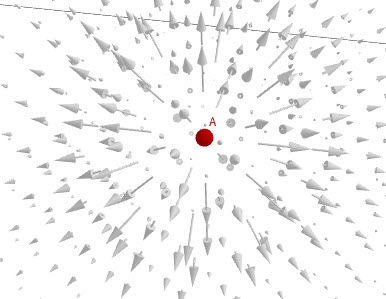
\includegraphics[scale=1]{../jpg/pointChargeField.jpg}
\end{center}
\caption{Electric field of a point charge}
\label{fig:eField}
\end{figure}




We want to find the magnitude of the electric field as a function of distance r from the charge. To do this, we will enclose the charge with an imaginary surface. We first have to decide on what kind of imaginary surface we are going to use in this case. Since the field has spherical symmetry, we will use a sphere, as shown in Figure \ref{fig:gaussPoint}. There are multiple reasons why we should use a sphere:

\begin{enumerate}
\item Symmetry of the charge dictates using a sphere.
\item The field on the sphere is in the same direction with the outward normal to the sphere.
\item Electric field is constant everywhere on the sphere.
\end{enumerate}




\begin{equation}
\oint_S \vec{E} \cdot \vec{dS} = \frac{Q_{inS}}{\epsilon}
\end{equation}



\begin{figure}[h!]
\begin{center}
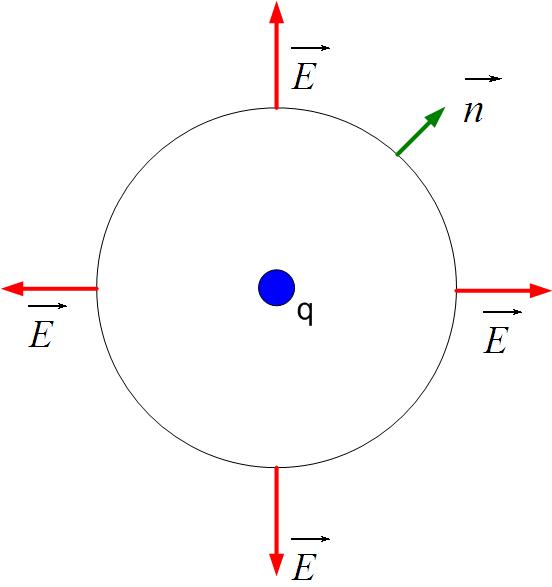
\includegraphics[scale=0.5]{../jpg/unitchargefield.jpg}
\end{center}
\caption{Application of Gauss's Law to find Electric Field of a point charge.}
\label{fig:gaussPoint}
\end{figure}

Because the electric field is in the same direction with the outward normal to the sphere as shown in Figure \ref{fig:gaussPoint}, the dot product becomes just the product of E and dS $\vec{E} \cdot \vec{dS}= E \,dS  \cos(\angle(\vec{E},\vec{dS}))= E \,dS  \cos(\angle(0^o)) =E dS$, and the Gauss's law equation becomes 



\begin{equation}
\oint_S E \,dS  = \frac{Q_{inS}}{\epsilon}
\end{equation}

Since the electric field is constant everywhere on the surface, we can take it out of the integral. 


\begin{equation}
 E \oint_S dS = \frac{Q_{inS}}{\epsilon}
\end{equation}

In the above equation the $\oint_S dS $ is just the surface area of the sphere, $4 \pi r^2$.


\begin{equation}
 E \, 4 \pi r^2 = \frac{Q_{inS}}{\epsilon}
\end{equation}

The final expression for the magnitude of the field is:


\begin{equation}
 E  = \frac{Q_{inS}}{4 \pi  \epsilon \, r^2}
\end{equation}

Note that we only found the magnitude of the field in the above equation. We started this problem with the knowledge of field radial direction. So the final expression for the field is

\begin{equation}
 \vec{E}  = \frac{Q_{inS}}{4 \pi  \epsilon \, r^2} \, \hat{r}
\end{equation}

Note that this equation can also be obtained from Coulomb's law. One last step in finding the electric field is to find the total charge enclosed by the imaginary surface S. Depending on whether we're looking for the field inside or outside of a charge distribution, and whether the charge distribution is a volume charge distribution $\rho$, surface charge distribution $\sigma$ or line charge distribution $\rho_l$, the whole or fraction of the volume V, surface S or line l of the charge distribution will be enclosed. 

\begin{eqnarray}
Q_{inS} = \int_V \rho \, dV \\
Q_{inS} =\int_S \sigma \, dS \\
Q_{inS} = \int_l \rho_l \, dl 
\end{eqnarray}

\subsection{Electric Field of a  Spherical Charge Distribution}


A spherical region of radius a is charged with uniform volume charge density $\rho$=const. Find the field inside the spherical region of charge at a distance r from the center of the charge density and the field outside of the spherical region of charge at (another) distance r away from the center of the charge.

\subsubsection{Electric Field outside of the sphere}

We will first look at the field  outside of the spherical charge distribution. This process is the same as in the previous problem where we found the field from a point charge. Following the reasoning in the previous problem we select a sphere for integration surface. It is important to mention that we pick a point outside of the distributed charge at the distance r from the center and that will be one point on the sphere's surface. We picked a point at random distance r, not at r=a, because we want to find out electric field anywhere outside of the charge distribution E(r), and r could be any point $r>a$. 

\begin{figure}[htbp]
\begin{center}
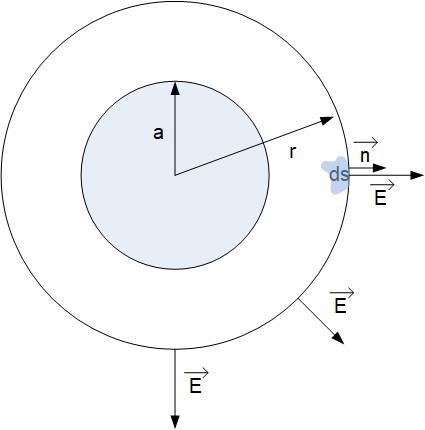
\includegraphics[scale=0.6]{../jpg/gaussSphereOut.jpg}
\end{center}
\caption{Application of Gauss's Law to find Electric Field of a spherical volume charge density.}
\label{fig:GaussSphereOut}
\end{figure}



\begin{equation}
\oint_S \vec{E} \cdot \vec{dS} = \frac{Q_{inS}}{\epsilon}
\end{equation}

Because the electric field is in the same direction with the outward normal to the sphere as shown in Figure \ref{fig:GaussSphereOut}, the dot product becomes just the product of scalars E and dS $\vec{E} \cdot \vec{dS}= E \,dS  \cos(\angle(\vec{E},\vec{dS}))= E \,dS  \cos(\angle(0^o)) =E dS$, and the Gauss's law equation becomes 

\begin{equation}
\oint_S E \,dS  = \frac{Q_{inS}}{\epsilon}
\end{equation}

Since the electric field is constant everywhere on the surface, we can take it out of the integral. 


\begin{equation}
 E \oint_S dS = \frac{Q_{inS}}{\epsilon}
\end{equation}

In the above equation the $\oint_S dS $ is just the surface area of the sphere, $4 \pi r^2$.


\begin{equation}
 E \, 4 \pi r^2 = \frac{Q_{inS}}{\epsilon}
\end{equation}

The final expression for the magnitude of the field is:


\begin{equation}
 E  = \frac{Q_{inS}}{4 \pi  \epsilon \, r^2}
\end{equation}

Note that we only found the magnitude of the field in the above equation. We started this problem with the knowledge of field radial direction. So the final expression for the field is

\begin{equation}
 \vec{E}  = \frac{Q_{inS}}{4 \pi  \epsilon \, r^2} \, \hat{r}
\end{equation}

Note that this equation can also be obtained from Coulomb's law. The charge $Q_{inS}$ is the total charge in the spherical volume where the charge is located. If the total charge in the volume was known, then this is the solution. However, in this problem, the charge density is known, so we have to find the total charge.

\begin{eqnarray}
Q_{inS}=\int_V \rho \, dV
\end{eqnarray}

Since the charge density $\rho$ is constant, it  can be taken outside of the integral.


\begin{eqnarray}
Q_{inS}=\rho \, \int_V \, dV
\end{eqnarray}

The integral above is then just the entire volume of the charge distribution, which is $V=\frac{4 \pi a^3}{3}$. The final expression for the electric field is 


\begin{eqnarray}
 \vec{E}  = \frac{\rho \, 4 \pi \, a^3}{12 \, \pi  \epsilon \, r^2} \, \hat{r} \\
 \vec{E}  = \frac{\rho \,   a^3}{3  \, \epsilon \, r^2} \, \hat{r}
\end{eqnarray}


Note that now the electric field is inversly proportional to the square of  distance from the center of the sphere, $E \sim 1/r^2$. The electric field decreases as we move away from the sphere.

\subsubsection{Electric field inside the sphere}




\begin{figure}[htbp]
\begin{center}
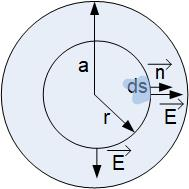
\includegraphics[scale=1]{../jpg/gaussSphereIn.jpg}
\end{center}
\caption{Application of Gauss's Law to find Electric Field of a .}
\label{fig:gaussSphereIn}
\end{figure}

Inside the spherical charge distribution, we'll again use a spherical imaginary surface  S to enclose charge, because of the spherical symmetry of the problem. The normal to the imaginary surface S is in the same direction with the electric field inside the spherical charge distribution as shown in Figure \ref{fig:gaussSphereIn}, and therefore the same analysis can be applied as above to get to conclusion that 



\begin{equation}
 E \, 4 \pi r^2 = \frac{Q_{inS}}{\epsilon}
\end{equation}




The difference in analysis here is if we look at the right side of Gauss's law  expression, because we now have to determine the amount of charge enclosed by the imaginary surface we created. The charge enclosed in the imaginary surface is not the total charge Q, it is a fraction of the total charge. What fraction of the charge is enclosed? It is the fraction of the charge in the volume enclosed by the by the surface S. 



\begin{eqnarray}
Q_{inS}=\int_V \rho \, dV
\end{eqnarray}

Since the charge density $\rho$ is constant, it  can be taken outside of the integral.


\begin{eqnarray}
Q_{inS}=\rho \, \int_V \, dV
\end{eqnarray}

The integral above is then just the fraction of the volume of the charge distribution enclosed by the surface S, which is $V=\frac{4 \pi r^3}{3}$. The final expression for the electric field is 


\begin{eqnarray}
 \vec{E}  = \frac{\rho \, 4 \pi \, r^3}{12 \, \pi  \epsilon \, r^2} \, \hat{r} \\
 \vec{E}  = \frac{\rho \, r}{3  \, \epsilon } \, \hat{r}
\end{eqnarray}

Note that now the electric field is proportional to the distance from the center of the sphere, $E\sim r$, the field increases from the center of the spere out until $r=a$. At $r=a$ the entire charge has been enclosed, and the field is maximum at that point.

\subsection{Electric field due to an infinite line of charge}


\begin{figure}[htbp]
\begin{center}
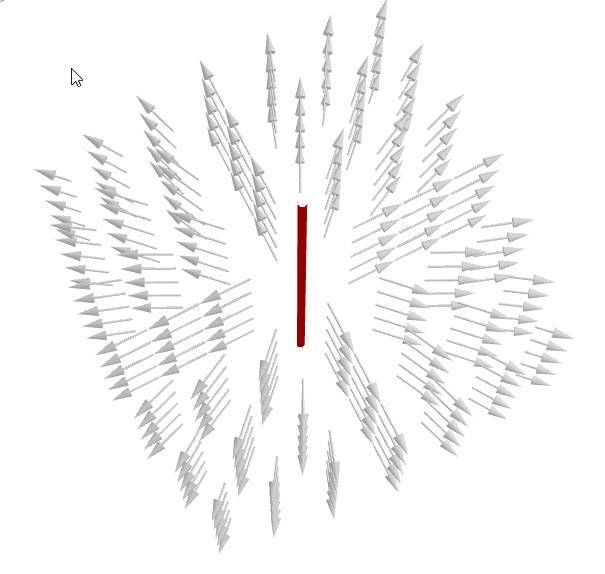
\includegraphics[scale=0.5]{../jpg/infiniteLineChargeField3D.jpg}
\end{center}
\caption{3-dimensional electric field of a wire.}
\label{GausLine}
\end{figure}


A cylindrical region of radius a and infinite length is charged with uniform volume charge density $\rho$=const and centered on the z-axis. Find the field inside the cylindrical region of charge at a distance r from the axis of the charge density and the field outside of the spherical region of charge at (another) distance r away from the z axis.

We will use Gauss's Law to solve this problem.



\subsubsection{Electric field outside the line of charge (a wire)}



 We first look at the field  outside of the cylindrical charge distribution. The wire is shown as a blue line in the direction of z-axis as shown in Figure \ref{fig:gaussLineOut}.  Because of the symmetry of the problem we select a cylinder for the closed surface S. It is important to mention that we pick a point outside of the distributed charge at the distance r from the z-axis. The point that we picked is one point on the sphere's surface. We picked a point from the z-axis at a distance r, not at r=a, because we want to find out electric field anywhere outside of the charge distribution E(r), and r could be any point $r>a$. Gauss's Law states that



\begin{figure}[htbp]
\begin{center}
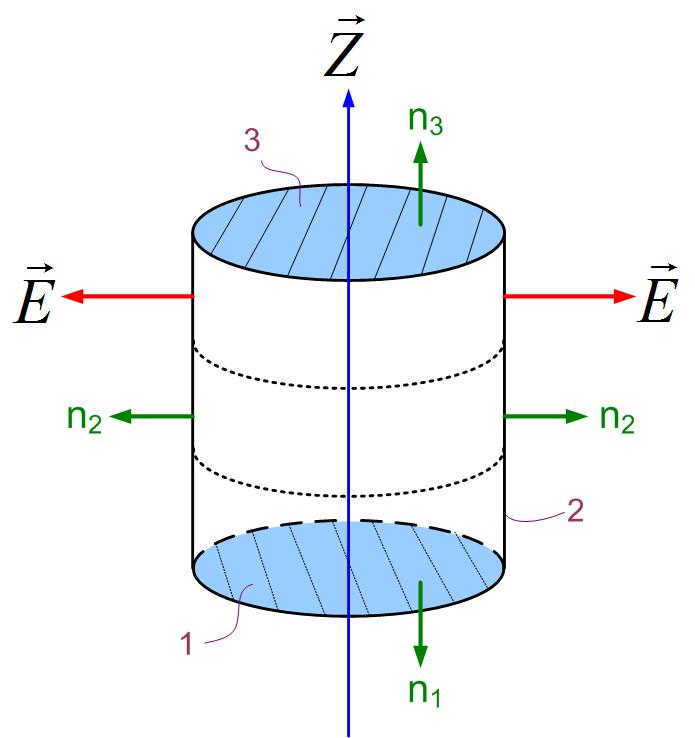
\includegraphics[scale=0.5]{../jpg/gausslawcylinder.jpg}
\end{center}
\caption{Application of Gauss's Law to find electric field of a wire.}
\label{fig:gaussLineOut}
\end{figure}




\begin{equation}
\oint_S \vec{E} \cdot \vec{dS} = \frac{Q_{inS}}{\epsilon}
\end{equation}


We will now apply Gauss's law to the three surfaces shown in Figure  \ref{fig:gaussLineOut}. The cylindrical surface consists of three surfaces: two bases S1 and S3 and the side surface S2. The normals to the bases are S1 and S3 are $\hat{n}_1=-\hat{z}$, $\hat{n}_3=\hat{z}$ and the normal to the side surface is  $\hat{n}_2=\hat{r}$. We can now split the flux of the electric field vector (the left-side of Gauss's law) through this closed cylindrical surface  intro three integrals:


 
\begin{equation}
\oint_S \vec{E} \cdot \vec{dS} = \int_{S1}  \vec{E} \cdot \vec{dS} +\int_{S2}  \vec{E} \cdot \vec{dS}+\int_{S3}  \vec{E} \cdot \vec{dS}
\end{equation}
 
 The electric field shown in Figure \ref{fig:gaussLineOut} is in the radial direction. The electric field lines only poke the side surface S2, and not surfaces S1 and S3. We therefore see that the flux through surfaces S1 and S3 is zero. This can also be shown mathematically. For the bases of the cylinder, the dot product between the top surface vector and the electric field vector in Gauss's law becomes $\vec{E} \cdot \vec{dS}= E \,dS  \cos(\angle(\vec{E},\vec{dS}))= E \,dS  \cos(\angle(90^o)) = 0$, and the Gauss's law equation becomes 

\begin{equation}
\int_{S2} E \,dS  = \frac{Q_{inS}}{\epsilon}
\end{equation}

Since the electric field is constant everywhere on the side surface, we can take it out of the integral. 


\begin{equation}
 E \int_{S2} dS = \frac{Q_{inS}}{\epsilon}
\end{equation}

In the above equation the $\int_{S2} dS $ is just the rectangular surface area of the side of the cylinder, $2 \pi r l$. Where r is the radius of the cylinder and l is the lenght of the cylinder.



\begin{equation}
 E \, 2 \pi r l = \frac{Q_{inS}}{\epsilon}
\end{equation}

From here we can find the magnitude of the field:


\begin{equation}
 E  = \frac{Q_{inS}}{2 \pi  \epsilon \, l\, r}
\end{equation}

Note that we only found the magnitude of the field in the above equation. We started this problem with the knowledge of the field's radial direction. 

\begin{equation}
 \vec{E}  = \frac{Q_{inS}}{2 \pi  \epsilon \, l\, r} \, \hat{r}
\end{equation}

 The charge $Q_{inS}$ is the total charge in the spherical volume where the charge is located. If the total charge in the volume was known, then this is the solution. However, in this problem, the charge density is known, so we have to find the total charge.

\begin{eqnarray}
Q_{inS}=\int_V \rho \, dV
\end{eqnarray}

Since the charge density $\rho$ is constant, it  can be taken outside of the integral.


\begin{eqnarray}
Q_{inS}=\rho \, \int_V \, dV
\end{eqnarray}

The integral above is then just the entire volume of the charge distribution, which is $V= a^2 \pi l$. The final expression for the electric field is 


\begin{eqnarray}
 \vec{E}  = \frac{\rho \, a^2 \pi l }{2 \, \pi  \epsilon \, l \,r} \, \hat{r} \\
 \vec{E}  = \frac{\rho \,   a^2}{2 \, \epsilon \, r} \, \hat{r}
\end{eqnarray}


Note that now the electric field is inversly proportional to the   distance from the z-axis, $E \sim 1/r$. The electric field decreases as we move away from the sphere, but slower than in the case of sphere of charge.


\subsubsection{Electric field inside the line of charge}

To find the electric field inside the cylindrical charge distribution, we zoom in the wire in the previous figure, and select a cylindrical imaginary surface S inside the wire, as shown in Figure \ref{fig:gaussLineIn}. Since electric field is in the same direction inside the wire, and the flux of the electric field is the same, we conclude that the left side of Gauss's law is the same as in the previous case. 


\begin{eqnarray}
E \, S = \frac{Q_{inS}}{\epsilon} \\
 E \, 2 \pi r l = \frac{Q_{inS}}{\epsilon}
\end{eqnarray}

The difference here is the amount of charge enclosed by the surface S.  



\begin{eqnarray}
Q_{inS}=\int_V \rho \, dV
\end{eqnarray}

Since the charge density $\rho$ is constant, it  can be taken outside of the integral.


\begin{eqnarray}
Q_{inS}=\rho \, \int_V \, dV
\end{eqnarray}

The integral above is then just the fraction of the volume of the charge distribution enclosed by the surface S, which is $V=r^2 \pi \, l $. The final expression for the electric field is 


\begin{eqnarray}
 \vec{E}  = \frac{\rho \, r^2 \, \pi  l }{2 \pi  l  \epsilon \, r} \, \hat{r} \\
 \vec{E}  = \frac{\rho \, r}{2  \, \epsilon } \, \hat{r}
\end{eqnarray}

The electric field is proportional to the distance from the center of the sphere, $E\sim r$, the field increases from the center of the spere out until $r=a$. At $r=a$ the entire charge has been enclosed, and the field is maximum at that point.




\begin{figure}[htbp]
\begin{center}
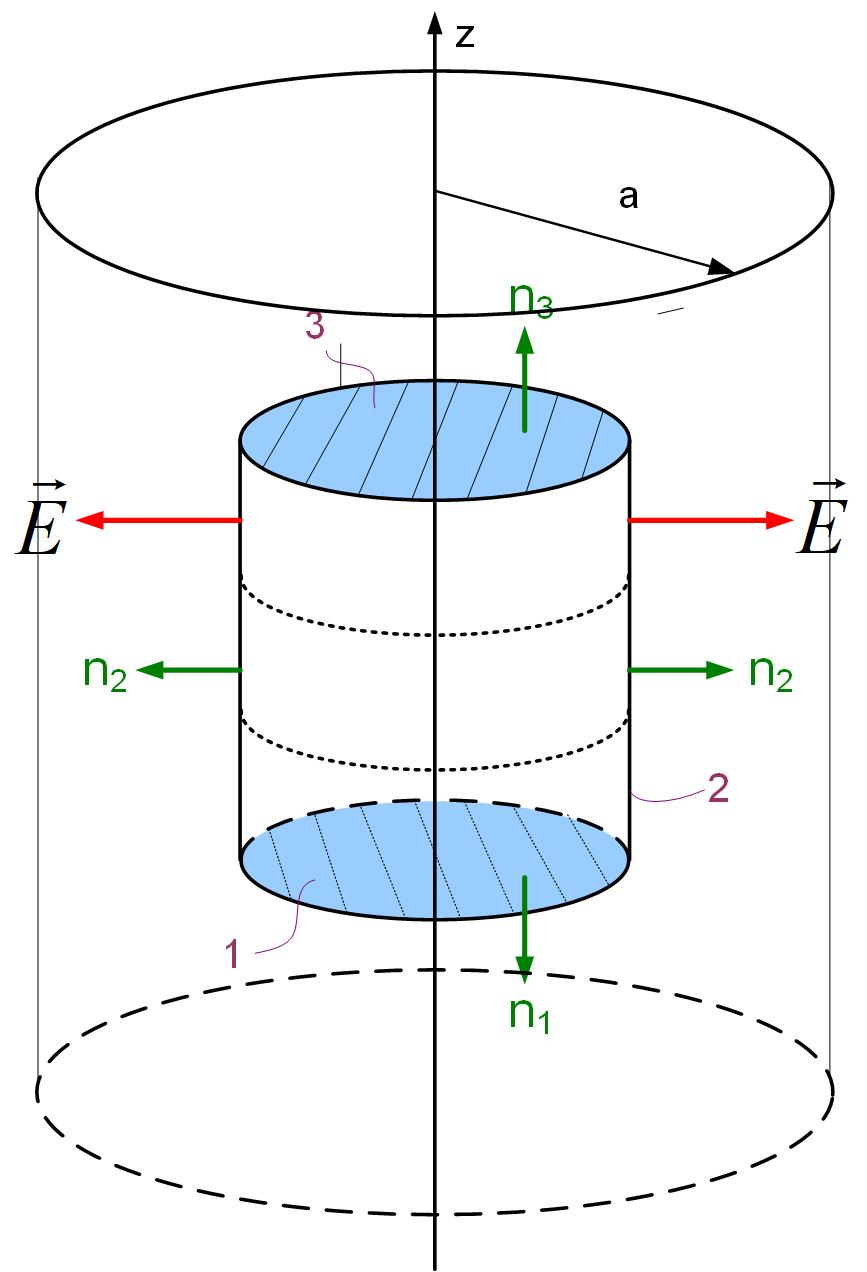
\includegraphics[scale=0.3]{../jpg/gausslawwireInside.jpg}
\end{center}
\caption{Infinite plane charged with positive surface charge density $\rho_S$.}
\label{fig:gaussLineIn}
\end{figure}


\subsection{Electric Field due to an infinite plane of Charge}

An infinite plane of charge has electric field in the direction away from it, as shown in Figure \ref{fig:3DFieldInfinitePlane}. In this figure the light blue plane represents the charged plane, and only electric field vectors are represented above the plane. Below the plane the vectors will be in the opposite direction, away from the plane. 


\begin{figure}[htbp]
\begin{center}
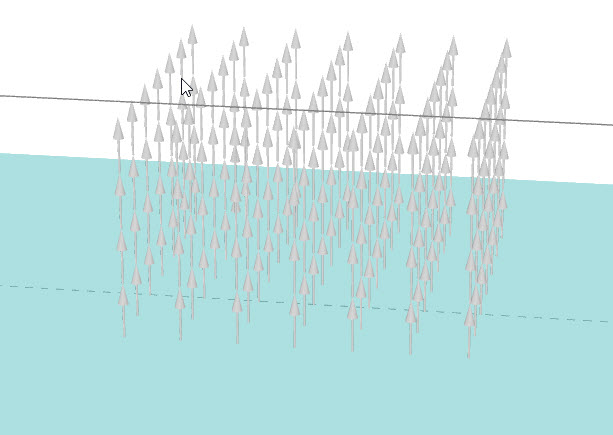
\includegraphics[scale=0.8]{../jpg/3DFieldInfinitePlane.jpg}
\end{center}
\caption{Electric field above an infinite plane charged with positive surface charge density $\rho_S$.}
\label{fig:3DFieldInfinitePlane}
\end{figure}


The flux of the electric field vector is zero for any frame that is perpendicular to the plane of charge. For our imaginary surface we can then use a box, where the flux will only exist through the top and bottom surfaces that are perpendicular to the field, or we can use a cylinder whose bases are parallel to the plane, as shown in Figure \ref{fig:gaussPlane}. 



\begin{figure}[htbp]
\begin{center}
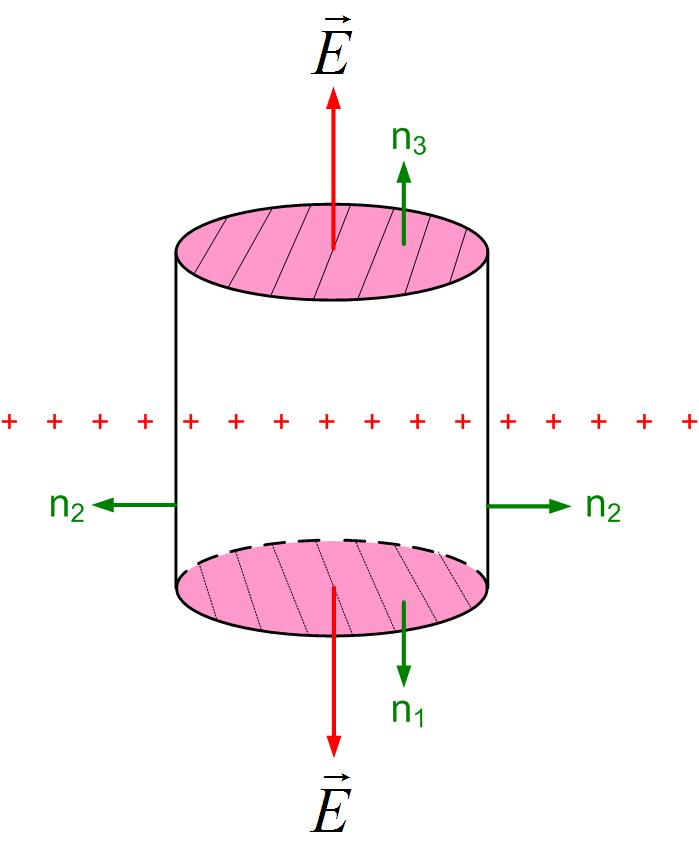
\includegraphics[scale=0.5]{../jpg/infiniteplaneofcharge.jpg}
\end{center}
\caption{Infinite plane charged with positive surface charge density $\rho_S$.}
\label{fig:gaussPlane}
\end{figure}


We can now separate the integral around the closed cylindrical surface to three surfaces, two that are parallel to the plane of charge, where flux is not zero, and one side surface where the flux is zero.

 
\begin{equation}
\oint_S \vec{E} \cdot \vec{dS} = \int_{S1}  \vec{E} \cdot \vec{dS} +\int_{S2}  \vec{E} \cdot \vec{dS}+\int_{S3}  \vec{E} \cdot \vec{dS} 
\end{equation}



 Mathematically the dot product between the electric field and the normal to the cylindrical top (S3) and bottom surface (S1) is just the product of the magnitudes of E and dS $\vec{E} \cdot \vec{dS}= E \,dS  \cos(\angle(\vec{E},\vec{dS}))= E \,dS  \cos(\angle(0^o)) =E dS$. The dot product on the side surface (S2) is zero, because the angle between the normal to the surface and the electric field is $90^o$, therefore the $\vec{E} \cdot \vec{dS}= E \,dS  \cos(\angle(\vec{E},\vec{dS}))= E \,dS  \cos(\angle(90^o)) =0$. We can subsequently take the electric field outside of the integral, and the integral around the closed surface then becomes
 
 

\begin{equation}
E \int_{S1} dS + E \int_{S2} dS = \frac{Q_{inS}}{\epsilon}
\end{equation}

 The integral of surface S1 and S1 is just the surface area of two surfaces.
 
\begin{eqnarray}
E \, S + E \, S = \frac{Q_{inS}}{\epsilon} \\
 2 E \,S = \frac{Q_{inS}}{\epsilon} \\
 E=\frac{Q_{inS}}{2 \epsilon S}
\end{eqnarray}

In the above equation, the ration $\frac{Q_{inS}}{S}$ is just the surface charge density $\sigma$. The final electric field expression for the infinite sheet of charge becomes

\begin{eqnarray}
 \vec{E}  = \pm \frac{\sigma}{2 \epsilon } \, \hat{z}
\end{eqnarray}

Note that in the above expression we added $\pm$ because we knew ahead of time the direction of the electric field. Below the z-axis it is in the negative z direction $-\hat{z}$, and above the z-axis it is in the positive z direction $\hat{z}$. Further, the electric field does not depend on the distance from the infinite plane, it is a constant that only depends on the surface charge density $\sigma$ and the dielectric permittivity of surrounding space $\epsilon$.

\subsection{Two Infinite Planes}


A parallel-plate capacitor can be modeled with two infinite, parallel plates of oposite charge densities. To find the total field we can use the principle of superposition, as shown in Figure \ref{Gaus2Plane}. The Figure shows first just the negative sheet of charge (the first region to the left), then, only the positive sheet of charge (region between two red vertical lines), and finally both sheets of charge in the region to the right. We first find the field separately for  the negative sheet of charge, then the positive sheet of charge, finally we sum them up to get the total field. 

In the previous section we found that the electric field from an infinite sheet of charge is constant. The electric field anywhere around the negative sheet of charge is

\begin{eqnarray}
 \vec{E_-}  = \mp \frac{\sigma}{2 \epsilon } \, \hat{z}
\end{eqnarray}

The electric field due to positive sheet of charge is


\begin{eqnarray}
 \vec{E_+}  = \pm \frac{\sigma}{2 \epsilon } \, \hat{z}
\end{eqnarray}

If you look at the direction of the field, the fields from individual plates between the plates of the capacitor add up, and the fields aboe and below the capacitor subtract. The final field is only between the plates of capacitor, and it is equal to double the value of the one sheet of charge.




\begin{eqnarray}
 \vec{E}  = \frac{\sigma}{ \epsilon } \, \hat{z}
\end{eqnarray}


\begin{figure}[htbp]
\begin{center}
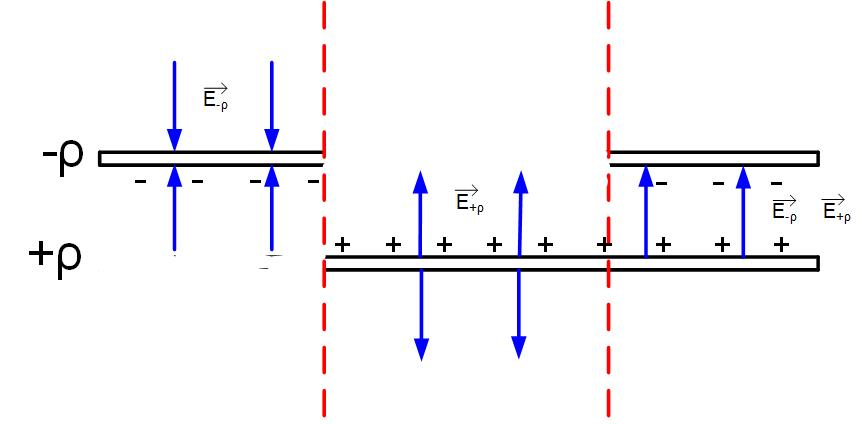
\includegraphics[scale=0.8]{../jpg/Infinite_Parallel_Plates1.jpg}
\end{center}
\caption{Two infinite planes charged with positive surface charge density $\rho_S$ and $-\rho_S.$}
\label{Gaus2Plane}
\end{figure}




\end{document} 
